\section{Algorithms for Learning a Policy Committee}
In this section, we present algorithmic approaches for train committee members to solve Problems~\ref{P:fix_K}.
%with respect to the desiderata formalized in Problems~\ref{P:fix_K} and~\ref{P:fix_delta}, which can be viewed as either goals in themselves (in some applications), or proxies for the general Objective~\ref{E:p2_alt} (in other applications).
We consider the special case of the problem in which the tasks have a \emph{structure representation}.
Specifically, we assume that each task can be represented using a parametric model $\psi_{\theta}(s,a)$, 
where the parameters $\theta \in \mathbb{R}^d$ comprise both of the parameters of the transition distribution $\mc{T}$ and reward function $r$.
Often, parametric task representation is given or direct; in cases when tasks are non-parametric, such as the Meta-World~\citep{yu2021metaworldbenchmarkevaluationmultitask}, we can often use approaches for task embedding, such as LLM-based task representations (see Section~\ref{S:llmembedding}).
%Such parametric task representations can be learned using a variety of task embedding methods in prior literature~\cite{}.
Consequently, we identify tasks $\tau$ with their representation parameters $\theta$ throughout, and overload $\Gamma$ to mean the distribution over task parameters, i.e., $\theta \sim \Gamma$.
%\luise{and when the goals are explicit, such as in morl/prl is a special case, the embedding will be shared across tasks and the diverse preferences/utility functions can be surveyed or learned eg. \cite{ge2024learning}?}

%We begin by considering a special case of MT-MDPs in which transition distributions $\mc{T}$ are shared by all tasks, which only differ in reward functions, and the reward functions are linear.
%For this setting, we propose algorithms with theoretical guarantees.
%Subsequently, we show how our algorithmic approaches can be applied to general MT-MDPs.



%\subsection{MT-MDPs with Linear Rewards}

%Consider MT-MDPs with linear rewards.
%Formally, we assume that $r_\tau(s,a) = \theta_\tau^T \phi(s,a)$ for a task-specific parameter vector $\theta_\tau \in \Theta$ and a shared reward embedding $\phi(s,a)$ (e.g., represented as a neural network), with $\Theta$ the set of reward function parameters.
%Since each task $\tau$ is associated with a vector $\theta_\tau \in \Theta$, we can equivalently refer to these vectors as representing tasks.
%We thus slightly abuse notation by having $\Gamma$ be the distribution over $\theta$ (task reward parameters).
%Linear rewards map naturally to the MORL setting with linear scalarization (with $\phi(s,a)$ in this case representing the vector of reward functions).
%Moreover, since embeddings $\phi(s,a)$ can be quite general, linearity is not as restrictive as it may at first seem.

\subsection{A High-Level Algorithmic Framework}

Even conventional RL presents a practical challenge in complex problems, as learning is typically time consuming and requires extensive hyperparameter tuning.
Consequently, a crucial consideration in algorithm design is to minimize the number of RL runs we need to obtain a policy committee.
To this end, we propose the following high-level algorithmic framework in which we only need $K$ independent (and, thus, entirely \emph{parallelizable}) RL runs.
%, where $K$ is a constant (Problem~\ref{P:fix_K}), or is explicitly minimized (Problem~\ref{P:fix_delta}).
This framework involves three steps:
\begin{enumerate}[leftmargin=*,topsep=0pt,itemsep=0pt]
    \item \textsc{Sample} $n$ tasks i.i.d. from $\Gamma$, obtaining $T=\{\theta_1,\ldots,\theta_n\}$ (parameters of associated tasks $\{\tau_1,\ldots,\tau_n\})$.
    In MTRL settings, $T$ is given.
    \item \textsc{Cluster} the task set $T$ into $K$ subsets, each with an associated representative $\theta_k$, and
    \item \textsc{Train} committee member $c_k\in \Pi$ for each cluster $k$ represented by $\theta_k$.
\end{enumerate}
As we shall see presently (and demonstrate experimentally in both Subsection~\ref{S:further} and Appendix~\ref{A:hist}), conventional clustering approaches are not ideally suited for our problem.
We thus propose several alternative approaches which yield theoretical guarantees on the quality of $\Pi$, in the special case that each committee member represents one policy.

% under mild conditions if all tasks share the transition dynamics and only differ in reward function.
Empirically, we show that the proposed framework outperforms state of the art even when tasks also have distinct transition distributions.

\subsection{Clustering}

The key aspect of our algorithmic design is clustering.
We are motivated by a connection between the clustering step (step (2) of the framework above) and efficacy of optimal policies learned for each cluster (step (3) of the framework), as a variant of simulation lemma~\citep{lobel2024optimal}, whose formal implications are discussed in the next section.
By leveraging a strong representation space, we can avoid the overhead of evaluating and clustering tasks on-policy and achieve high efficacy with minimal computational cost.
Thus, we focus on the following problem instead: 

%This, in turn, provides us with a clustering objective that would yield formal guarantees about the efficacy of the policy committee we thereby obtain in the special case $c_k=\pi_k.$

%Indeed, our framework aims to minimize the computational cost while achieving high efficacy.    Hence, by relying on a good representation space we avoid the overhead to evaluate and cluster the tasks on-policy, so that we just solve the following problem instead. Note the connection between Problem~\ref{P:fix_K} and Problem \ref{P:fix_K_C} is backed by Lemma~\ref{thm:linear_reg} in the next section.


\begin{definition}
\label{D:cluster_cover}
A set of representatives $C=\{\theta_1,\ldots,\theta_K\}$ is an \emph{$(\epsilon,1-\delta)$-parameter-cover} for a \emph{task distribution} $\Gamma$ if $\min_{\theta' \in C}\|\theta - \theta'\|_\infty \le \epsilon$ with probability at least $1-\delta$ with respect to $\theta \sim \Gamma$.  
%$C$ is an \emph{$(\epsilon,1-\delta)$-parameter-cover} for \emph{a set of tasks} $\{\tau_1,\ldots,\tau_n\}$ if $\min_{\theta' \in C}\|\theta - \theta'\|_\infty \le \epsilon$ for at least a fraction $1-\delta$ of tasks $\theta \in T$.
\end{definition}

\begin{problem}
    \label{P:fix_K_C}
    Fix $K$ and $\epsilon$.  Our goal is to find $C$ with $|C| \le K$ which is a $(\epsilon,1-\delta)$-parameter-cover for the smallest $\delta \in [0,1]$.
\end{problem}


Notably, while conventional clustering techniques, such as k-means, can be viewed as proxies for these objectives, there are clear differences insofar as the typical goal is to minimize sum of shortest distances of \emph{all} vectors from cluster representatives, whereas our goal, essentially, is to ``cover" as many vectors as we can. In Appendix ~\ref{A:hist}, we provide a histogram of individual task returns to illustrate the different impact the two clustering methods make.

We show next that our problem is strongly inapproximable, \emph{even if we restrict attention to $K=1$}.
\begin{definition}[\textsc{Max-1-Cover}]
    Let $T = \{\theta_1,\ldots,\theta_n\} \subseteq \mathbb{R}^d$. Find $\theta \in \mathbb{R}^d$ which maximizes the size of $S \subseteq T$ with $\max_{\theta' \in S}\|\theta - \theta'\|_\infty \le \epsilon$.
%    Find a set  in $R^d$, we would like to cover as many $\theta_i$ using one $\Tilde{\theta}$ so that every $\theta_i$ covered by $\Tilde{\theta}$ will be within $\epsilon$ distance.
\end{definition}
\begin{theorem}\label{thm:NPhard}
    For any $\epsilon > 0$ \textsc{Max-1-Cover}  does not admit an $n^{1-\epsilon}$ -approximation unless P = NP.
\end{theorem}
We prove this in Appendix~\ref{A:NP} via an approximation-preserving reduction from the Maximum Clique problem~\citep{engebretsen2000clique}.
Despite this strong negative result, we next design two effective algorithmic approaches.
The first method runs in polynomial time with a constant $d$, and provides a constant-factor approximation.
The second is a general gradient-based approach.

\noindent\textbf{Greedy Elimination Algorithm (GEA) }
Before we discuss our main algorithmic approaches, we begin with GEA, which provides a useful building block, but not theoretical guarantees.
Consider a set $T$ of task parameter vectors, fix $K$, and suppose we wish to identify an $(\epsilon,1-\delta)$-parameter-cover with the smallest $\delta$ (Problem~\ref{P:fix_K_C}), but restrict attention to $\theta \in T$ in constructing such a cover.
This problem is an instance of a \textsc{Max-K-Cover} problem (where subsets correspond to sets covered by each $\theta \in T$), and can be approximated using a greedy algorithm which iteratively adds one $\theta \in T$ to $C$ that maximizes the most uncovered vectors in $T$.
Its fixed-$\delta$ variant, on the other hand, is a set cover problem if $\delta = 0$, and a similar greedy algorithm approximates the minimum-$K$ cover $C$ for any $\delta$.
\iffalse
\begin{algorithm}[h]
    \caption{Greedy Elimination}
    \label{alg:greedy_elimination}
    \textbf{Input}: $T = \{\theta_i\}_{i=1}^N$, $\epsilon > 0$, $K \ge 1$ \\
    \textbf{Output}: Parameter cover $C$
    \begin{algorithmic}[1]
    \STATE $C \gets []$
        \FOR{$round\ k$ = $1$ to $K$}
            \STATE 
              \STATE $\hat{\theta}_k \gets $ 
            \STATE $T \gets T - covered$
            \STATE $C$.adds($\hat{\theta}_k$)
        \ENDFOR
        \STATE \textbf{return} $C$
    \end{algorithmic}
\end{algorithm}
\fi
However, neither of these algorithms achieves a reasonable approximation guarantee (as we can anticipate from Theorem~\ref{thm:NPhard}), although our experiments show that greedy elimination is nevertheless an effective heuristic.
But, as we show next, we can do better if we allow cluster covers $\theta$ to be unrestricted.

\noindent\textbf{Greedy Intersection Algorithm (GIA) }
We now present our algorithm which yields provable approximation guarantees when task dimension is low.
The key intuition behind GIA is that for any $\theta$, a $\epsilon$-hybercube centered at $\theta$ characterizes all possible $\theta'$ that can cover $\theta$ in the sense of Definition~\ref{D:cluster_cover}. Thus, if any pair of $\epsilon$-hypercubes centered at $\theta$ and $\theta'$ intersects, any point at the intersection covers both.
To illustrate, consider the following simple example:
%To see it more clearly, we provide the following example in the one-dimensional setting:


\begin{center}
    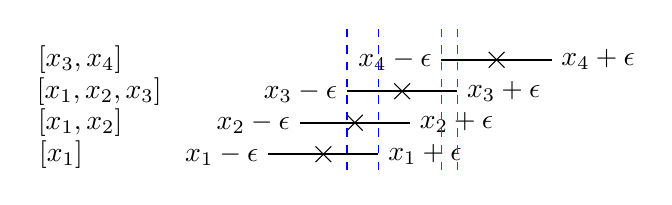
\begin{tikzpicture} [scale=2]

\def\cross{%
    \draw (-0.05,-0.05) -- (0.05,0.05);
    \draw (-0.05,0.05) -- (0.05,-0.05);
}

    
% First line segment
\draw[thick] (0,0) coordinate (A) -- (0.7,0) coordinate (B);
\draw (A) node[left] {$[x_1] \hspace{1.3cm} x_1-\epsilon$};
\draw (B) node[right] {$x_1+\epsilon$};

{%
    \draw (0.35-0.05,-0.05) -- (0.35+0.05,0.05);
    \draw (0.35-0.05,0.05) -- (0.35+0.05,-0.05);
}

% Second line segment
\draw[thick] (0.2,0.2) coordinate (C)-- (0.9,0.2)coordinate (D);
\draw (C) node[left] {$[x_1,x_2] \hspace{1.2cm} x_2-\epsilon$};
\draw (D) node[right] {$x_2+\epsilon$};

{%
    \draw (0.55-0.05,0.2-0.05) -- (0.55+0.05,0.2+0.05);
    \draw (0.55-0.05,0.2+0.05) -- (0.55+0.05,0.2-0.05);
}



\draw[thick] (0.5,0.4) coordinate (E) -- (1.2,0.4) coordinate (F);
\draw (E) node[left] {$[x_1,x_2,x_3] \hspace{1.3cm} x_3-\epsilon$};
\draw (F) node[right] {$x_3+\epsilon$};
{%
    \draw (0.85-0.05,0.4-0.05) -- (0.85+0.05,0.4+0.05);
    \draw (0.85-0.05,0.4+0.05) -- (0.85+0.05,0.4-0.05);
}


\draw[thick] (1.1,0.6) coordinate (I) -- (1.8,0.6) coordinate (J);
\draw (I) node[left] {$[x_3,x_4] \hspace{3cm} x_4-\epsilon$};
\draw (J) node[right] {$x_4+\epsilon$};

{%
    \draw (1.45-0.05,0.6-0.05) -- (1.45+0.05,0.6+0.05);
    \draw (1.45-0.05,0.6+0.05) -- (1.45+0.05,0.6-0.05);
}
\draw[dashed,red] (1.1,-0.1) -- (1.1,0.8);
\draw[dashed,red] (1.2,-0.1) -- (1.2,0.8);
\draw[dashed,blue] (0.7,-0.1) -- (0.7,0.8);
\draw[dashed,blue] (0.5,-0.1) -- (0.5,0.8);


\end{tikzpicture}
\end{center}

Each cross represents a parameter we aim to cover, while each line segment indicates the possible locations of the $\epsilon$-close representative for that parameter. 
By selecting a point within the overlapping region of these intervals, we can effectively cover their parameters simultaneously.



%consider a toy example with two thetas $\theta_1,\theta_2$. Every point inside the $\epsilon$-hypercube centered at $\theta_1$, can be a representative of $\theta_1$ since their distance is bounded by $\epsilon.$ Hence, if the  $\epsilon$-hypercubes centered at $\theta_1$, $\theta_2$ have an intersection, then any point at the intersection can cover both $\theta_1$ and $\theta_2$.

%So in order to find the best coverage, we may want to construct an entire intersection tree but then the complexity would be exponential in $n$ in the worst case because when we include a new datapoint $\theta_i$ to the tree, we need to consider its intersection with every possible intersection formed by the previous datapoints, with rank $0$ to $i-1$. The total number of new intersections to check is $ \sum_{k=0}^{i-1}=
%\begin{pmatrix}
%    i-1 \\k
%\end{pmatrix} =2^{i-1}$. And it would require $\sum_{k=1}^{n}2^{k-1}=2^n-1$ checking steps to establish the whole intersection tree.\\

\iffalse
This may lead to a naive idea of iteratively constructing an intersection tree for all $\theta \in T$.
Unfortunately, the size of such a tree is exponential in $n$ in the worst case because we need to check the intersection between every subset of parameters. 
\fi
%Instead, we propose a \textsc{Greedy Intersection} algorithm, which is polynomial in $n$ that gets around this issue. 
The proposed \textsc{GIA} algorithm generalizes this intuition as follows.
The first stage of the algorithm is to create an intersection tree for each dimension independently. For $s$-th dimension, we sort the datapoints' $s$-th coordinates in ascending order.
%, which takes $\log(n)$ time by MergeSort. 
We refer to the sorted coordinates as $x_1 < x_2 \dots <x_n$, and create a list for each point $x_i$ to remember how many other points can be covered together with it with initialization being $[x_i]$ itself.

Starting from the second smallest datapoint $x_2$, we check if $x_2-\epsilon \le x_1+\epsilon,$ i.e. if $x_2\le x_1+2\epsilon.$ Since $x_2-\epsilon>x_1-\epsilon$ due to our sorting, any point inside $[x_2-\epsilon,x_1+\epsilon]$ can cover both $x_1,x_2.$ Therefore if this interval is valid, we add $x_1$ to the list $[x_2]$ to indicate the existence of a simultaneous coverage for $x_1,x_2$. In general, for $x_i$, we check if $x_i \le x_j +2\epsilon$ with a descending $j=i-1 $ to $1$ or until the condition no longer holds. If the inequality is satisfied, we add $x_j$ to $x_i$'s list. Then since we have ordered the set, for every index $j' $ less than $j$, $x_i > x_j+2\epsilon> x_{j'}+2\epsilon.$ The coverage for all the $x$ in $x_i$'s list would be the interval $[x_i-\epsilon, x_j+\epsilon],$ where $j$ is the smallest index in $x_i$'s list.
There are $1+2+\dots+n-1= \mathcal{O}(n^2)$ comparisons in total. 
We form a set of these lists, and call it $\mathcal{A}_s$ for the $s$-th dimension. The figure above illustrates how the algorithm works to find out $\mathcal{A}_1= \{[x_1],[x_1,x_2],[x_1,x_2,x_3], [x_4,x_5]\}$. 
\iffalse
\begin{center}
    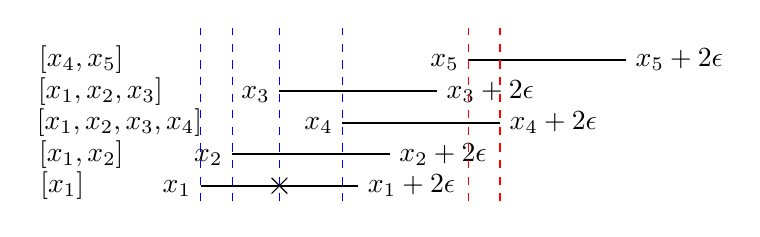
\begin{tikzpicture} [scale=2]

\def\cross{%
    \draw (-0.05,-0.05) -- (0.05,0.05);
    \draw (-0.05,0.05) -- (0.05,-0.05);
}

    
% First line segment
\draw[thick] (0,0) coordinate (A) -- (1,0) coordinate (B);
\draw (A) node[left] {$[x_1] \hspace{1cm} x_1$};
\draw (B) node[right] {$x_1+2\epsilon$};

{%
    \draw (0.5-0.05,-0.05) -- (0.5+0.05,0.05);
    \draw (0.5-0.05,0.05) -- (0.5+0.05,-0.05);
}

% Second line segment
\draw[thick] (0.2,0.2) coordinate (C)-- (1.2,0.2)coordinate (D);
\draw (C) node[left] {$[x_1,x_2] \hspace{0.9cm} x_2$};
\draw (D) node[right] {$x_2+2\epsilon$};


% Third line segment
\draw[thick] (0.9,0.4) coordinate (E) -- (1.9,0.4) coordinate (F);
\draw (E) node[left] {$[x_1,x_2,x_3,x_4] \hspace{1.3cm} x_4$};
\draw (F) node[right] {$x_4+2\epsilon$};

% Fourth line segment
\draw[thick] (0.5,0.6) coordinate (G) -- (1.5,0.6) coordinate (H);
\draw (G) node[left] {$[x_1,x_2,x_3] \hspace{1cm} x_3$};
\draw (H) node[right] {$x_3+2\epsilon$};

% Fifth line segment
\draw[thick] (1.7,0.8) coordinate (I) -- (2.7,0.8) coordinate (J);
\draw (I) node[left] {$[x_4,x_5] \hspace{3.9cm} x_5$};
\draw (J) node[right] {$x_5+2\epsilon$};



\draw[dashed,red] (1.7,-0.1) -- (1.7,1);
\draw[dashed,red] (1.9,-0.1) -- (1.9,1);
\draw[dashed,blue] (0.0,-0.1) -- (0.0,1);
\draw[dashed,blue] (0.2,-0.1) -- (0.2,1);
\draw[dashed,blue] (0.5,-0.1) -- (0.5,1);
\draw[dashed,blue] (0.9,-0.1) -- (0.9,1);
\end{tikzpicture}
\end{center}
\fi






The second stage is to find a hypercube covering the most points, consisting of an axis from each dimension. 
%Due to 
By the geometry of the Euclidean space, 
%we know that 
two points $\theta_1,\theta_2$ are within $\epsilon$ in $\ell_\infty$-distance iff they appear inside one's list together for each dimension. Therefore, in order to find the maximum coverage with one hypercube such that its center is within $\ell_\infty$-distance to the most points, we wonder which combination of lists, $l_1 \dots l_d$
each from the sets $\mathcal{A}_1 \dots \mathcal{A}_d $ produces an intersection of the maximum cardinality. In our example, we can conclude that $[x_1,x_2,x_3], [x_4,x_5]$ need to be covered separately by two points between the blue or red vertical lines.

The full algorithm is provided in Appendix~\ref{S:code}.
%(see Algorithm~\ref{alg:greedy_intersection} there).
%Algorithm~\ref{alg:greedy_intersection} formalizes this discussion.\luise{Move the pseudocode to the appendix?}
%Unfortunately, the general form of this problem has been studied under \cite{clifford2011maximum}, which shows that solving the problem is NP hard and has a hard approximation.
%Note that this approach can be used both when $K$ is fixed, and when we wish to minimize $K$ to achieve $1-\delta$ coverage of $T$: the only difference is whether we stop iterating when we reach the budget in the number of clusters, or $1-\delta$ coverage.
Next, we show that \textsc{GIA} yields provable coverage guarantees.
We defer the proof to Appendix~\ref{A:greedy_gaurantee}.
For these results we use \textsc{GIA}($K$) to refer to the solution (set $C=\{\theta_1,\ldots,\theta_K\}$) returned by \textsc{GIA}.
%\textsc{Greedy Intersection} algorithm.
%with a fixed $K$, while \textsc{GI}($\delta$) refers to the solution $C$ returned by this algorithm which continues until achieving $1-\delta$ coverage of $T$.


\begin{theorem}\label{thm:greedy_gaurantee}
Suppose $T$ contains $n \ge \frac{9\log({5/\alpha})}{2\beta^2}$ i.i.d.~samples from $\Gamma$.
Let $1-\delta^*(K,\epsilon)$ be the optimal coverage of a $\epsilon$-parameter-cover of $\Gamma$ under fixed $K,\epsilon$.
%\luise{We should change the uncertainty parameter $\delta$ to a different letter}
Then with probability at least $1-\alpha$, 
\textsc{GIA}($K$) is a $(\epsilon,(1-\frac{1}{e})(1-\delta^*(K,\epsilon)-K\beta))$-parameter-cover of $\Gamma$.
%Under sample complexity $\mathcal{O}(\frac{1}{\epsilon^2}\log\delta), $ with probability at least $1-\delta$, the policy committee of size $K$ we constructed after collecting the samples can cover a task from the same distribution with probability $(1-\frac{1}{e})({OPT}-K\epsilon)$ .
\end{theorem}



The key limitation of \textsc{GIA} is that it is exponential in $d$, and thus requires the dimension to be constant.
This is a reasonable assumption in some settings, such as low-dimensional control.
%MORL settings, where the set of reward functions one is concerned with is typically small, whereas the set of possible scalarizations (which comprise the set of tasks in our setting) is continuous, and thus the sufficient sample size $n$ is likely large.
However, in many other settings, both $n$ and $d$ can be large.
Our next algorithm addresses this issue.

\noindent\textbf{Gradient-Based Coverage }
Consider Problem~\ref{P:fix_K_C}.
For a finite set $T$, we can formalize this as the following optimization problem:
%We can use a similar idea to approximately solve the full $K$-coverage problem.
%Specifically, consider the following optimization problem, which represents our goal:
\begin{align}
\label{E:optK}
    \max_{\{\theta_1,\ldots,\theta_K\}} \sum_{\theta \in T} \mathbf{1}(\min_{k \in [K]} \|\theta_{k}-\theta\|_\infty \le \epsilon),
\end{align}
where $\mathbf{1}(\cdot)$ is 1 if the condition is true and 0 otherwise.
%We can also use this to solve Problem~\ref{P:fix_delta_C} using a binary search over $K$, since coverage is non-decreasing in $K$.
However, objective~\eqref{E:optK} is non-convex and discontinuous.
To address this, we propose the following differentiable proxy:
%Now, we can relax this problem in a similar manner:
\begin{align}
\label{E:relaxK}
    \min_{\substack{\{\theta_1,\ldots,\theta_K\};\\\alpha \in \mathbb{R}^{nK}}} \sum_i \mathbf{ReLU}\left(\left\{\sum_{k=1}^K \sigma_k(\alpha_{i})\|\theta_{k}-\theta_i\|_\infty\right\} -\epsilon\right),
\end{align}
where $\sigma(\cdot)$ is a softmax function.
Next, we demonstrate that this is a principled proxy by showing that when full coverage of $T$ is possible, solutions of~\eqref{E:optK} and~\eqref{E:relaxK} coincide. The proof is in Appendix~\ref{A:softmax}.
\begin{theorem} \label{thm:softmax}
    Fix $K$ and suppose $\exists \theta \in \{\theta_1,\ldots,\theta_K\}$ such that $\|\theta-\theta_i\| \le \epsilon$ for all $i$.  Then the sets of optimal solutions to \eqref{E:optK} and \eqref{E:relaxK} are equivalent.
\end{theorem}
Thus, we can use gradient-based methods with objective in~\eqref{E:relaxK} to approximate solutions to 
%either 
Problem~\ref{P:fix_K_C}. 
Because the objective is still non-convex, we can improve performance by initializing with the solution obtained using \textsc{GEA} or \textsc{GIA}
%\textsc{Greedy Elimination} or \textsc{Greedy Intersection} 
when $d$ is low.

%\luise{An extension to the above is online policy committee formation.}



\subsection{Theoretical Analysis for MTRL}

We now put things together by showing that we have a sample efficient approach for learning a policy committee $\Pi$ which achieves a $(\epsilon,1-\delta)$-cover for $\Gamma$.
For this result, we focus on the special case where each committee member is one fixed policy and assume that each task has a shared dynamics, and a parametric reward function $r_\theta(s,a)$ where $\theta$ identifies a task-specific reward.
While this is a theoretical limitation, we note that our subsequent clustering and training algorithms do not in themselves require this assumption, and our experimental results demonstrate that the overall approach is effective generally.

Let $\pi_i^*$ denote the optimal policy for task $\pi_i$.
We use $V_i^{\pi_j^*}$ to denote the value of task $\tau_i$ using a policy that is optimal for task $\tau_j$.
\begin{lemma}\label{thm:linear_reg}
Suppose that $r_\theta(s,a)$ is $L$-Lipschitz in $L_\infty$ norm, that is, for all $\theta, \theta'$, $\sup_{s,a}|r_\theta(s,a)-r_{\theta'}(s,a)| \le L \|\theta - \theta'\|_\infty$.
Then, for any two tasks $\tau_i$ and $\tau_j$ with respective $\theta_i$ and $\theta_j$ that satisfy $\|\theta_i-\theta_j\|_\infty \le \epsilon$,
$V_i^{\pi_j^*} \ge V_i^{\pi_i^*} - 2L\frac{1-\gamma^{h+1}}{1-\gamma} \epsilon$ if $\gamma < 1$ and $V_i^{\pi_j^*} \ge V_i^{\pi_i^*} - 2Lh\epsilon$ if $\gamma = 1$.
%\begin{align*}
%V_i^{\pi_j^*} &\ge V_i^{\pi_i^*} - 2L\frac{1-\gamma^{h+1}}{1-\gamma} \epsilon &\mathrm{if}& \quad \gamma < 1, \quad \mathrm{and}\\
%V_i^{\pi_j^*} &\ge V_i^{\pi_i^*} - 2Lh\epsilon &\mathrm{if}& \quad \gamma = 1.
%\end{align*}
\end{lemma}
See Appendix~\ref{A:simmulation} for proof. Lipschitz continuity is a mild assumption; for example, it is satisfied by ReLU neural networks.

%Next, we connect this to our ultimate goal as expressed in Problem~\ref{P:fix_K}.
%and~\ref{P:fix_delta}.

\begin{comment}
    \begin{definition}
\label{D:cluster_cover}
A set of representatives $C=\{\theta_1,\ldots,\theta_K\}$ is an \emph{$(\epsilon,1-\delta)$-parameter-cover} for a \emph{task distribution} $\Gamma$ if $\min_{\theta' \in C}\|\theta - \theta'\|_\infty \le \epsilon$ with probability at least $1-\delta$ with respect to $\theta \sim \Gamma$.  
%$C$ is an \emph{$(\epsilon,1-\delta)$-parameter-cover} for \emph{a set of tasks} $\{\tau_1,\ldots,\tau_n\}$ if $\min_{\theta' \in C}\|\theta - \theta'\|_\infty \le \epsilon$ for at least a fraction $1-\delta$ of tasks $\theta \in T$.
\end{definition}
\end{comment}





\begin{comment}
The following result then follows directly from Lemma~\ref{thm:linear_reg}.
\begin{theorem}
\label{thm:param_cover}
    Suppose $C$ is an \emph{$(\epsilon,1-\delta)$-parameter-cover} for $\Gamma$ and $r_\theta(s,a)$ is $L$-Lipschitz in $L_\infty$, and let $\Pi$ contain a set of optimal policies to each $\theta \in C$.
    Then $\Pi$ is a \emph{$(2L\frac{1-\gamma^{h+1}}{1-\gamma} \epsilon,1-\delta)$-cover} for $\Gamma$ when $\gamma < 1$ and \emph{$(2Lh\epsilon,1-\delta)$-cover} when $\gamma=1$.\footnote{We note that this and other results also work for the FS-MT-MDP setting with a finite set of tasks $T$. We omit this from the results for easier readability.}
\end{theorem}

\end{comment}

%This result enables us to focus on obtaining $(\epsilon,1-\delta)$-parameter-cover guarantees \emph{solely in the space of policy parameters}, at least when policies all share dynamics and differ only in reward functions.

Next, we combine Theorem~\ref{thm:greedy_gaurantee} and Lemma~\ref{thm:linear_reg} to conclude that we can compute a policy committee $\Pi$ which provides provable coverage guarantees for a task distribution $\Gamma$ with polynomial sample complexity.
\begin{theorem}\label{thm:greedy_gaurantee_final}
Suppose $T$ contains $n \ge \frac{9\log({5/\alpha})}{2\beta^2}$ i.i.d.~samples from $\Gamma$ and $r_\theta(s,a)$ is $L$-Lipschitz in $L_\infty$.
Let $1-\delta^*(K,\epsilon)$ be the optimal coverage of a $\epsilon$-parameter-cover of $\Gamma$ under fixed $K,\epsilon$, and suppose that for any task $\tau$ we can find a policy $\pi$ with $V^\pi \ge V_\tau^* - \eta$.
%\luise{We should change the uncertainty parameter $\delta$ to a different letter}
Then we can compute a committee $\Pi$
 which is a $(2L\frac{1-\gamma^{h+1}}{1-\gamma} \epsilon + \eta,(1-\frac{1}{e})(1-\delta^*(K,\epsilon)-K\beta))$ for $\Gamma$ when $\gamma < 1$ and $(2Lh\epsilon+\eta,(1-\frac{1}{e})(1-\delta^*(K,\epsilon)-K\beta))$ for $\Gamma$ when $\gamma=1$  with probability at least $1-\alpha$.
%Under sample complexity $\mathcal{O}(\frac{1}{\epsilon^2}\log\delta), $ with probability at least $1-\delta$, the policy committee of size $K$ we constructed after collecting the samples can cover a task from the same distribution with probability $(1-\frac{1}{e})({OPT}-K\epsilon)$ .
\end{theorem}



%\textbf{I took the sample complexity from Lemma 7 proof, but it is not clear what $\delta$ means there.  Is this $\delta^*(K)$?}\luise{Oh, the $\delta$ in the proof is a different}

\subsection{Few-Shot Adaptation}

\label{S:fewshot}
A particularly useful consequence of learning a policy committee $\Pi$ that is a $(\epsilon,1-\delta)$-cover is that we can leverage it in meta-learning for few-shot adaptation. The algorithmic idea is straightforward: evaluate each of $K$ policies in $\Pi$ by computing a sample average sum of rewards over $N$ randomly initialized episodes, and choose the best policy $\pi \in \Pi$ in terms of empirical average reward.
%This yields the following sample complexity bound.

In particular, suppose that $\gamma = 1$.
We now show that this translates into a few-shot sample complexity on a previously unseen task $\tau$ that is linear in $K$ (the size of the committee). Details of the proof are in Appendix~\ref{A:adaptation}.
%\begin{definition}
    %We define the best expert as $\pi^* = \mathrm{argmax}_{\pi\in \Pi} V^{\pi}$, the expert which yields the highest expected average cumulative reward $V^{\pi}$ from its steady-state  $\mu_\pi$. The cumulative regret, $r(n)$ after $n$ iterations of a multi-armed bandit algorithm is defined as: $r(n)=nV^{*}-\sum_{k=0}^{n}\frac{1}{T_k}\sum_{t=t_k}^{t_{k+1}-1} r_t$ By Theorem~\ref{thm:linear_reg} $V^{\pi*}$ is at least $2LT\epsilon-$optimal to $V*$ since $V^{\pi*} \ge V^{\pi'} $ where $\pi'\in \Pi$ is inside the cover.\end{definition}

%\begin{theorem}(Regret decomposition identity). If the induced Markov chains for each policy committee member $\pi \in \Pi$ are irreducible and aperiodic, then the expected cumulative regret at time n can be bounded with:$\mathbb{E}[r(n)] \le \sum \mathbb{E}[T(n)][\delta_\pi+\frac{C_\pi}{T_0(1-\beta_pi)}]+\frac{C_*}{}(1-\beta_*)\sum_{k=0}^{n-1}\frac{1}{T_k}$ \end{theorem}


%TODO: formal bounds for few-shot adaptation; idea 1: $K$ policy evaluation steps followed by playing the best policy; what is the bound on regret?  How does it compare to regret bounds in standard RL?  Is there a UCB bound that we can use and treat policies in $\Pi$ as ``experts''? 

%Having solved the committee formation problem, we can now utilize the RLPA algorithm to quickly identify the best policy member in the committee with regret bound measured \emph{against the optimal policy for the underlying MDP}, rather than by the best policy in the committee.

%One application 


\iffalse
We can then leverage \emph{online learning} approaches which treat $\Pi$ as a set of policy \emph{experts}.
To illustrate, we can use the RLPA algorithm due to \citet{azar2013regret}, which combined with our methods above can yield provable regret bounds, as we show next.


\fi

\iffalse
\begin{theorem}\citep{azar2013regret}
\label{T:regret}
   Let $f$ be an increasing function and $S^+$ the span of the best policy in $\Pi$ with average reward $\mu_\Pi^*$.
   Under Assumption~\ref{A:online}, for any number of trials $N \ge f^{-1}(S^+)$ the regret of the RLPA algorithm with $K$ deterministic policies with respect to $\mu_\Pi^*$ is bounded by
$\Delta(s)\le 24(f(N)+1)\sqrt{3NK(\log(N/\alpha))}+\sqrt{N} +6f(N)K(\log_2(S^+)+2\log_2(N))$
with probability at least $1-\alpha$ for any initial state $s \in \mathcal{S}$.
\end{theorem}




\begin{corollary}\label{cor:RLPA}
Suppose $\Pi$ with $|\Pi|=K$ is an $(\epsilon,1-\delta)$-cover for $\Gamma$. Then under Assumption~\ref{A:online}, with probability at least $1-\delta-\alpha$, for any number of trials $N \ge f^{-1}(S^+)$, the regret of a  task $\tau \sim \Gamma$ with respect to the optimal average reward $\mu^* = V_\tau^*/h$ for $\tau$ is bounded by
$\Delta(s)\le 24(f(N)+1)\sqrt{3NK(\log(N/\alpha))}+\sqrt{N} +6f(N)K(\log_2(N^+)+2\log_2(N))+\frac{\epsilon}{h}$, for any $s\in \mathcal{S}$.
\end{corollary}
A notable aspect of this result is that while conventional regret in online learning, such as in Theorem~\ref{T:regret}, is measured with respect to the best policy in the (small) set of experts, we obtain low regret with respect to the \emph{optimal} policy for the task faced at execution time.
This is the key consequence of the committee $\Pi$ constituting a $(\epsilon,1-\delta)$ cover.
\fi

%on the efficacy of policy committees.
%For small $K$,  Azuma’s inequality have guaranteed us high confidence that we can also evaluate each policy repeatedly and select the one with the highest reward.

%We now connect this result with the notion of $(\epsilon,1-\delta)$-cover that we have, noting that $V^\pi_\tau = h\mu^\pi_\tau$ for any $\pi,\tau$.
\begin{theorem}\label{thm:online_repetition}
Suppose $\Pi$ is a $(\epsilon,1-\delta)$-cover for $\Gamma$ and let $\tau \sim \Gamma$. Under some mild conditions,
if we run 
%the number of episodes ran for each policy 
$p \ge\frac{32h(H+1)^2\log(4/\alpha)}{(\beta-2H)^2}$ episodes for each policy $\pi \in \Pi$, where $H$ is a constant, the policy $\pi$ that maximizes the empirical return yields $V_\tau^\pi \ge V_\tau^* -\epsilon-\beta$ with probability at least $1-\delta-\alpha$, where $V_\tau^*$ is the optimal reward for $\tau$.
\end{theorem}

%\vspace{-15pt}

%\vspace{-5pt}
%While this result assumes that each policy $\pi \in \Pi$ has been fixed for the duration of adaptation (that is, we are only doing policy evaluation for each), in practice a simple improvement is to actually fine-tune each policy as we get more experience.
%This is the variation that we use in the experiments below.

%Notably, this suggests that a simple few-shot learning algorithm in which we perform policy evaluation for each of $K$ policies, and then use the one with the best empirical performance, will lead to effective few-shot learning.



\subsection{Training}


The output of the \textsc{Clustering} step above is a set of representative task parameters $C = \{\theta_1,\ldots,\theta_K\}$.
The simplest way to use these to obtain a policy committee $\Pi$ is to train a policy $\pi_k$ optimized for each $\theta_k \in C$.
However, this ignores the set of tasks that comprise each cluster $k$ associated with a representative $\theta_k$ (i.e., the set of tasks closest to $\theta_k$). 
As demonstrated empirically in the multi-task RL literature, using multiple tasks to learn a shared representation facilitates generalization (effectively enabling the model to learn features that are beneficial to all tasks in the cluster)~\citep{sodhani2021multi,sun2022paco,yang2020multi}. 
%In addition, Ruder (2017) further highlights that training on multiple related tasks can improve performance by reducing overfitting to any single task and fostering more robust representations
%They may help with the generalization as the previous multi-task learning literature has pointed out.
%Moreover, training policies on imaginary tasks may not be feasible (in which case we can use the Greedy Elimination approach).

To address this, we propose an alternative which trains a policy $\pi_k$ to maximize the sum of rewards of the tasks in cluster $k$.
Notably, our approach can use \emph{any} RL algorithm to learn a policy associated with a cluster of tasks; in the experiments below, we use the most effective MTRL or meta-RL baseline for this purpose.


The RL problem itself will typically dominate computational complexity in practice, but in cases where RL can be efficiently learned~\citep{brafman2002r,kearns2002near} and dimension $d$ is constant, we additional have polynomial algorithmic complexity.

\iffalse
The limitation of the approaches above is that they are still connected only to the task representations $\theta$, rather than tasks themselves.



To address this, we propose to add an \emph{policy evaluation} step in each RL iteration that removes tasks covered by the policies learned thus far \emph{in terms of their values}, rather than $\ell_\infty$ similarity, and only trains a policy $\pi_k$ on the residual members of the cluster $k$.

While this yields a more precise evaluation of committee efficacy, it is also considerably slower 
%(as it interjects policy evaluation steps between RL rounds at each step $k$), 
and not as easily parallelizable.
\fi

\subsection{Dealing with Non-Parametric Tasks}
\label{S:llmembedding}

Our approach assumes that tasks are parametric, so that we can reason (particularly in the clustering step) about parameter similarity.
Many practical multi-task settings, however, are non-parametric, so that our algorithmic framework cannot be applied directly.
In such cases, our approach can make use of any available method for extracting a parametric representation of an arbitrary task $\tau$.
For example, it is often the case that tasks can be either described in natural language.
We propose to leverage this property and use text embedding (e.g., from pretrained LLMs) as the parametric representation of otherwise non-parametric tasks, where this is feasible.
Our hypothesis is that this embedding captures the most relevant semantic aspects of many tasks in practice, a hypothesis that our results below validate in the context of the Meta-World benchmark.
This is analogous to what was done by \citet{bing2023meta}, with the main difference being that our task descriptions are with respect to higher-level goals, whereas \citet{bing2023meta} describe tasks in terms of associated plans.
%To handle tasks without a clear parametric representation (such as Metaworld) we generate a parameterzations from a pretrained LLM as follows. First we provide a string to the LLM of the form: "Task name: objective: Environmental Details:".
%For example:
%As an illustration, consider the \emph{Window-Open} task in Meta-World.
%We can describe this task as follows:
%\begin{quote}
%\textit{``Objective: Slide a window open. Environmental Details: The window is set within a frame and can slide horizontally. The robot must apply lateral force to slide the window open. Window positions are randomized."}
%\end{quote}
We provide the full list of task descriptions for the Meta-World environment in Appendix~\ref{S:llmdesc}. 